% !TEX root = ../../main.tex

\section{Calorimetry dataset UiO-66(Zr)}

\begin{figure}[H]
    \centering

    \begin{subfigure}{0.25\linewidth}
        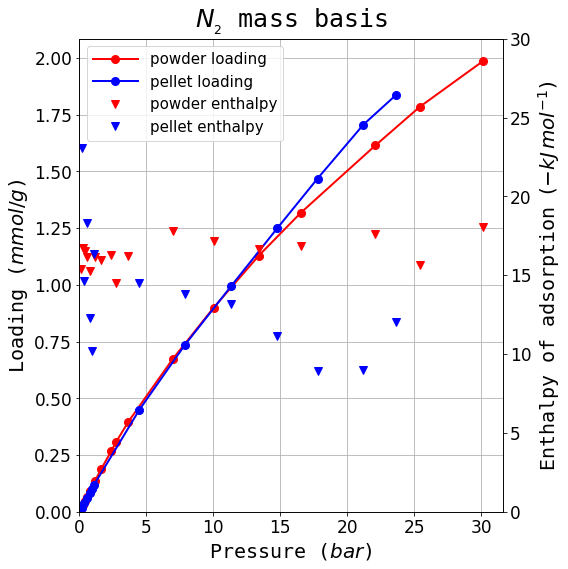
\includegraphics[width=\textwidth]{calo/UiO-66(Zr)/nitrogen-mass-basis-iso}%
        \label{appx:fig:shaping:uio66n2mass}
    \end{subfigure}%
    \begin{subfigure}{0.25\linewidth}
        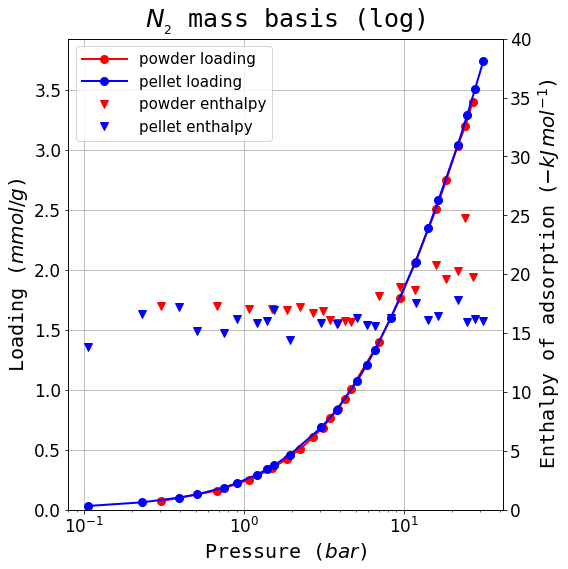
\includegraphics[width=\textwidth]{calo/UiO-66(Zr)/nitrogen-mass-basis-log-iso}%
        \label{appx:fig:shaping:uio66n2masslog}
    \end{subfigure}%
    \begin{subfigure}{0.25\linewidth}
        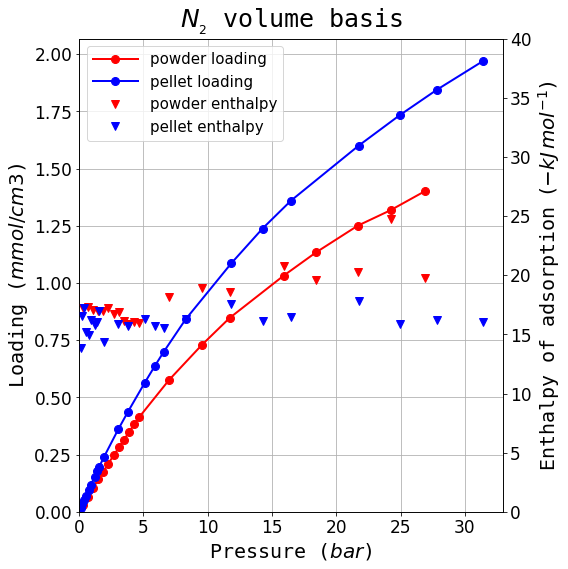
\includegraphics[width=\textwidth]{calo/UiO-66(Zr)/nitrogen-volume-basis-iso}%
        \label{appx:fig:shaping:uio66n2volume}
    \end{subfigure}%
    \begin{subfigure}{0.25\linewidth}
        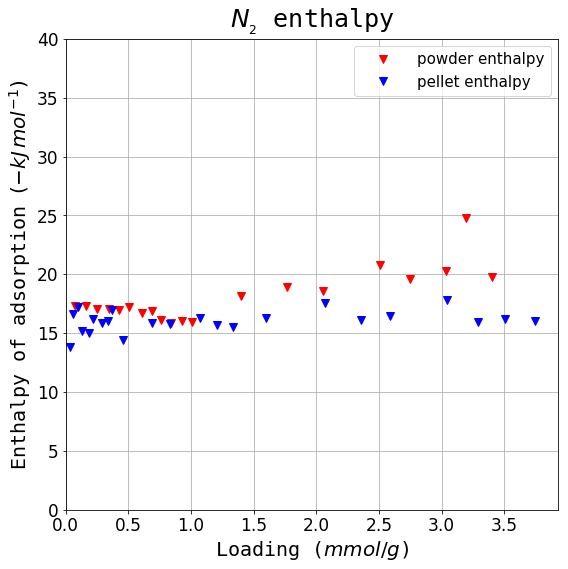
\includegraphics[width=\textwidth]{calo/UiO-66(Zr)/nitrogen-enth}%
        \label{appx:fig:shaping:uio66n2enth}%
    \end{subfigure}%

    \begin{subfigure}{0.25\textwidth}
        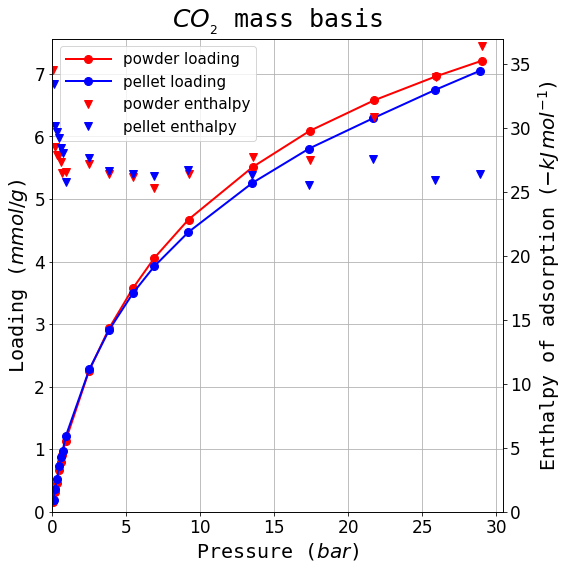
\includegraphics[width=\textwidth]{calo/UiO-66(Zr)/carbondioxide-mass-basis-iso}%
        \label{appx:fig:shaping:uio66co2mass}
    \end{subfigure}%
    \begin{subfigure}{0.25\textwidth}
        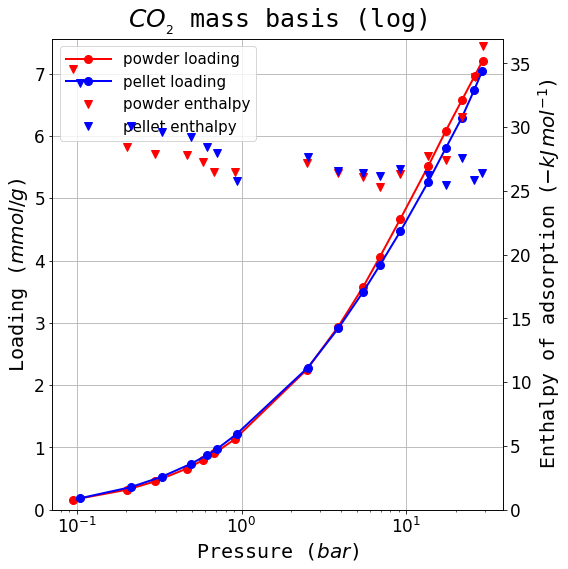
\includegraphics[width=\textwidth]{calo/UiO-66(Zr)/carbondioxide-mass-basis-log-iso}%
        \label{appx:fig:shaping:uio66co2masslog}
    \end{subfigure}%
    \begin{subfigure}{0.25\textwidth}
        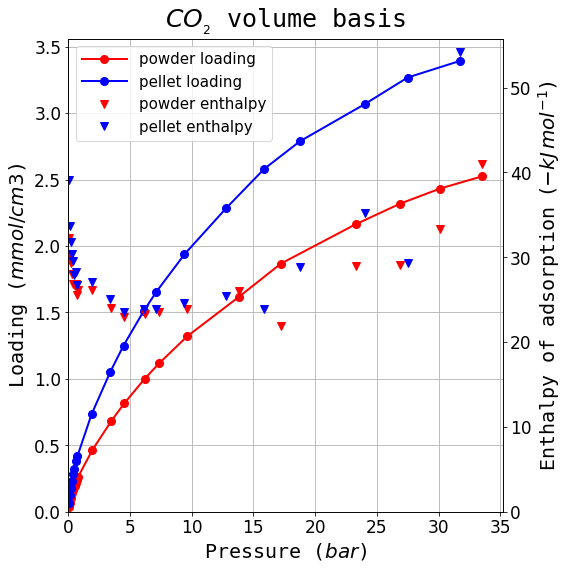
\includegraphics[width=\textwidth]{calo/UiO-66(Zr)/carbondioxide-volume-basis-iso}%
        \label{appx:fig:shaping:uio66co2volume}
    \end{subfigure}%
    \begin{subfigure}{0.25\textwidth}
        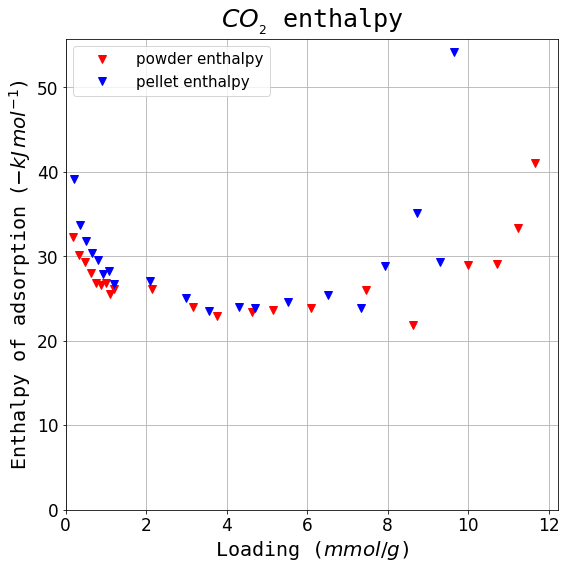
\includegraphics[width=\textwidth]{calo/UiO-66(Zr)/carbondioxide-enth}%
        \label{appx:fig:shaping:uio66co2enth}%
    \end{subfigure}%

    \begin{subfigure}{0.25\textwidth}
        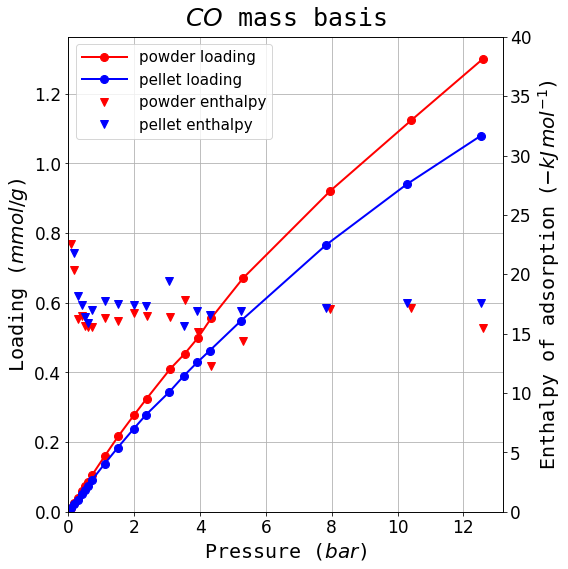
\includegraphics[width=\textwidth]{calo/UiO-66(Zr)/carbonmonoxide-mass-basis-iso}%
        \label{appx:fig:shaping:uio66comass}
    \end{subfigure}%
    \begin{subfigure}{0.25\textwidth}
        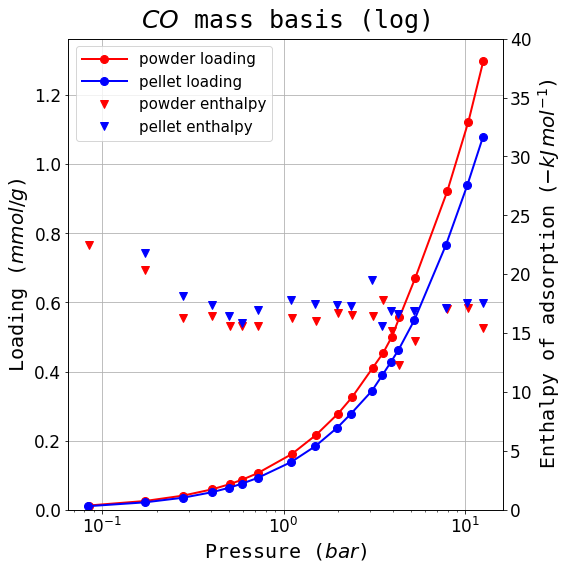
\includegraphics[width=\textwidth]{calo/UiO-66(Zr)/carbonmonoxide-mass-basis-log-iso}%
        \label{appx:fig:shaping:uio66comasslog}
    \end{subfigure}%
    \begin{subfigure}{0.25\textwidth}
        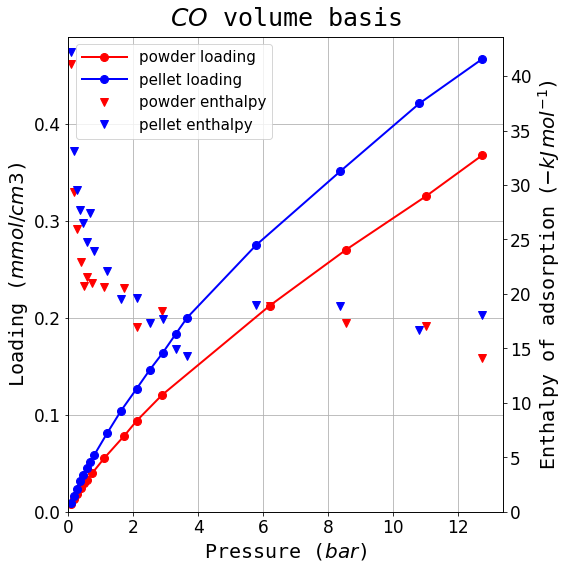
\includegraphics[width=\textwidth]{calo/UiO-66(Zr)/carbonmonoxide-volume-basis-iso}%
        \label{appx:fig:shaping:uio66covolume}
    \end{subfigure}%
    \begin{subfigure}{0.25\textwidth}
        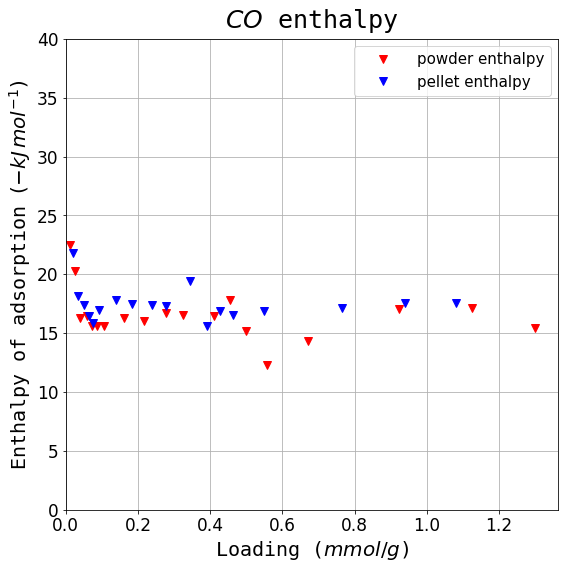
\includegraphics[width=\textwidth]{calo/UiO-66(Zr)/carbonmonoxide-enth}%
        \label{appx:fig:shaping:uio66coenth}%
    \end{subfigure}%

    \begin{subfigure}{0.25\textwidth}
        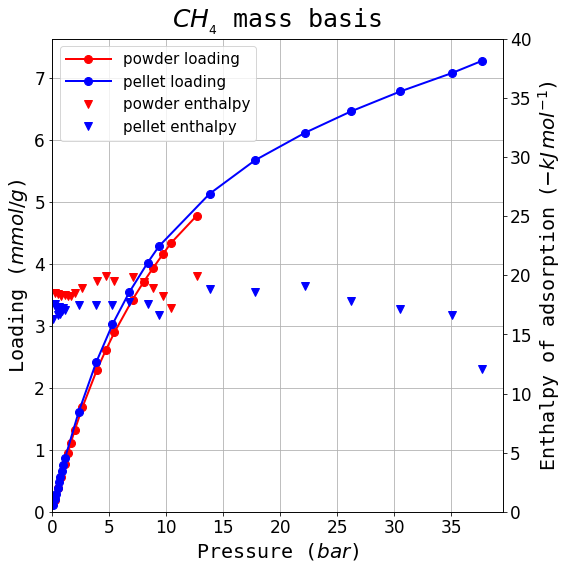
\includegraphics[width=\textwidth]{calo/UiO-66(Zr)/methane-mass-basis-iso}%
        \label{appx:fig:shaping:uio66ch4mass}
    \end{subfigure}%
    \begin{subfigure}{0.25\textwidth}
        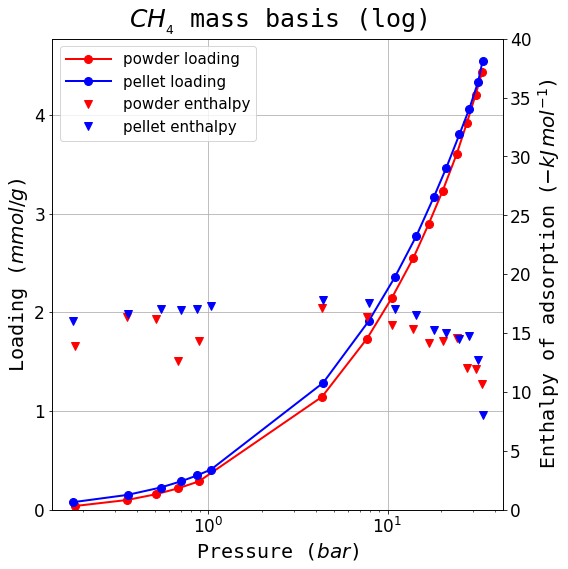
\includegraphics[width=\textwidth]{calo/UiO-66(Zr)/methane-mass-basis-log-iso}%
        \label{appx:fig:shaping:uio66ch4masslog}
    \end{subfigure}%
    \begin{subfigure}{0.25\textwidth}
        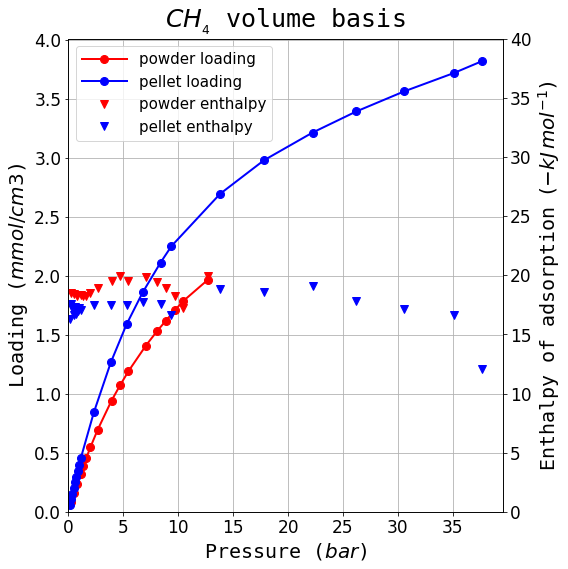
\includegraphics[width=\textwidth]{calo/UiO-66(Zr)/methane-volume-basis-iso}%
        \label{appx:fig:shaping:uio66ch4volume}
    \end{subfigure}%
    \begin{subfigure}{0.25\textwidth}
        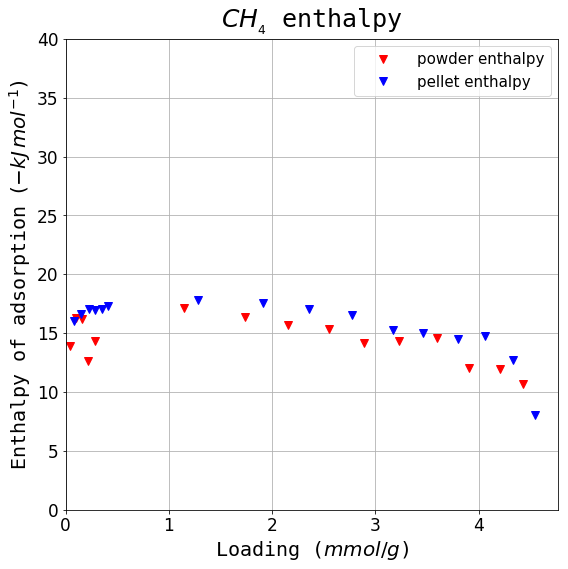
\includegraphics[width=\textwidth]{calo/UiO-66(Zr)/methane-enth}%
        \label{appx:fig:shaping:uio66ch4enth}%
    \end{subfigure}%

    \caption{Complete isotherm and enthalpy dataset for UiO-66(Zr)}
\end{figure}

\begin{figure}[H]

    \begin{subfigure}{0.25\textwidth}
        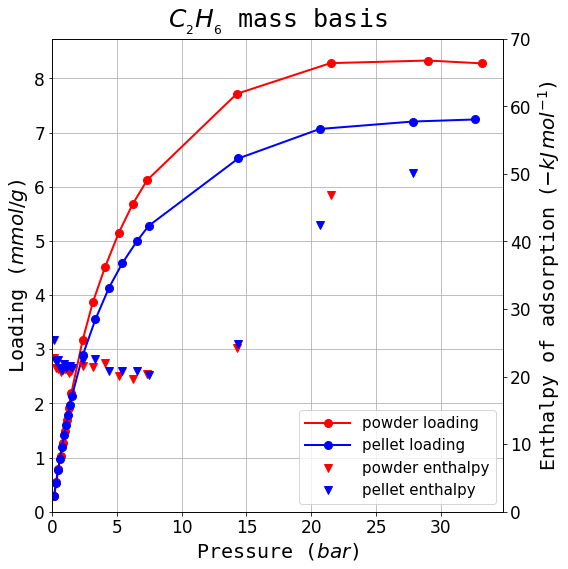
\includegraphics[width=\textwidth]{calo/UiO-66(Zr)/ethane-mass-basis-iso}%
        \label{appx:fig:shaping:uio66c2h6mass}
    \end{subfigure}%
    \begin{subfigure}{0.25\textwidth}
        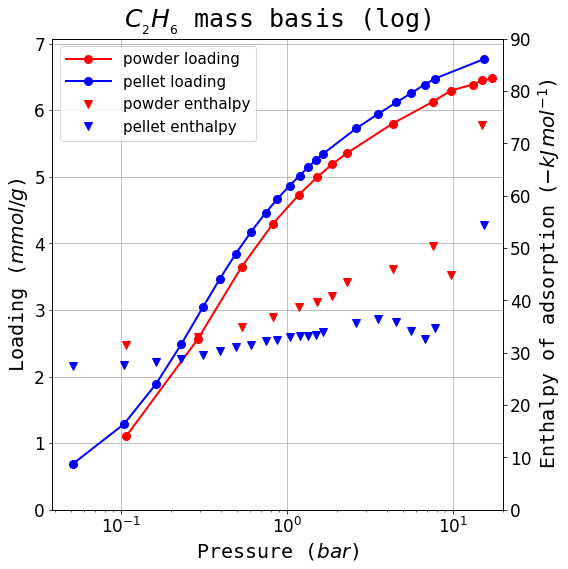
\includegraphics[width=\textwidth]{calo/UiO-66(Zr)/ethane-mass-basis-log-iso}%
        \label{appx:fig:shaping:uio66c2h6masslog}
    \end{subfigure}%
    \begin{subfigure}{0.25\textwidth}
        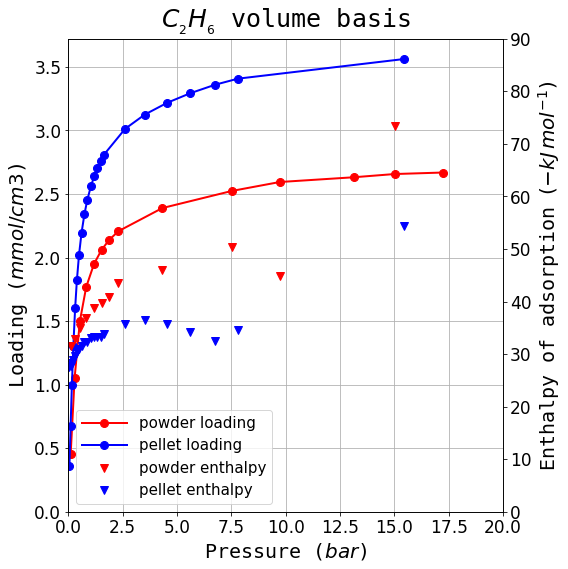
\includegraphics[width=\textwidth]{calo/UiO-66(Zr)/ethane-volume-basis-iso}%
        \label{appx:fig:shaping:uio66c2h6volume}
    \end{subfigure}%
    \begin{subfigure}{0.25\textwidth}
        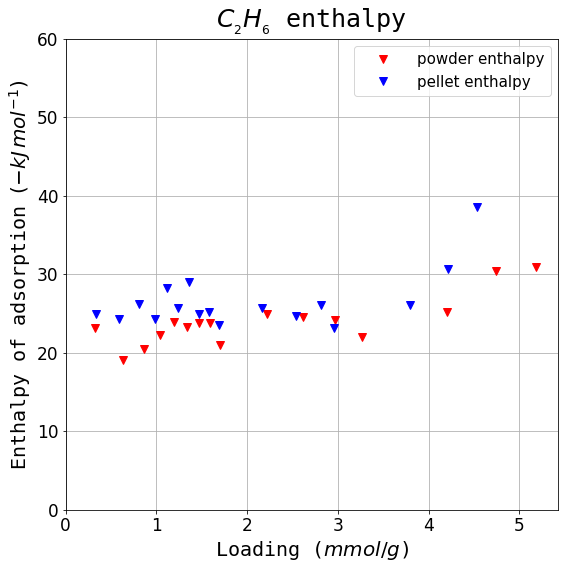
\includegraphics[width=\textwidth]{calo/UiO-66(Zr)/ethane-enth}%
        \label{appx:fig:shaping:uio66c2h6enth}%
    \end{subfigure}%

    \begin{subfigure}{0.25\textwidth}
        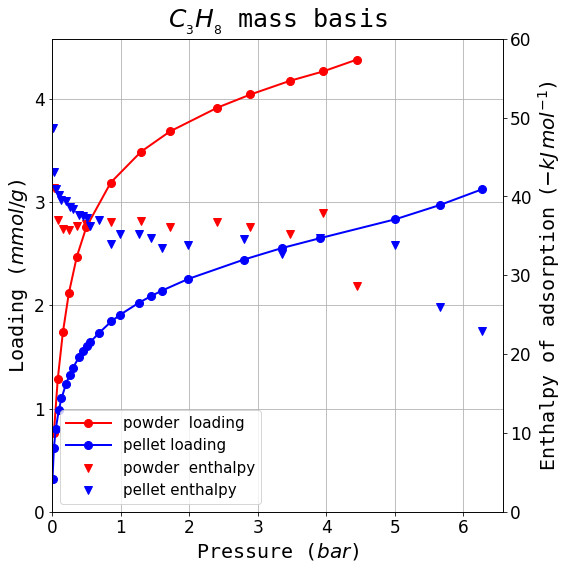
\includegraphics[width=\textwidth]{calo/UiO-66(Zr)/propane-mass-basis-iso}%
        \label{appx:fig:shaping:uio66c3h8mass}
    \end{subfigure}%
    \begin{subfigure}{0.25\textwidth}
        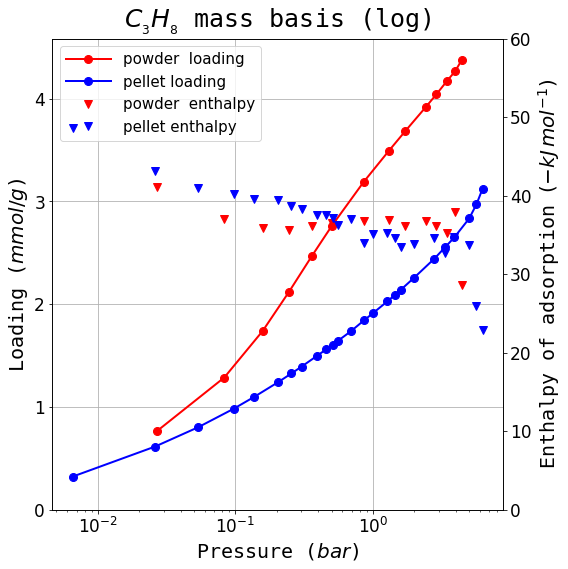
\includegraphics[width=\textwidth]{calo/UiO-66(Zr)/propane-mass-basis-log-iso}%
        \label{appx:fig:shaping:uio66c3h8masslog}
    \end{subfigure}%
    \begin{subfigure}{0.25\textwidth}
        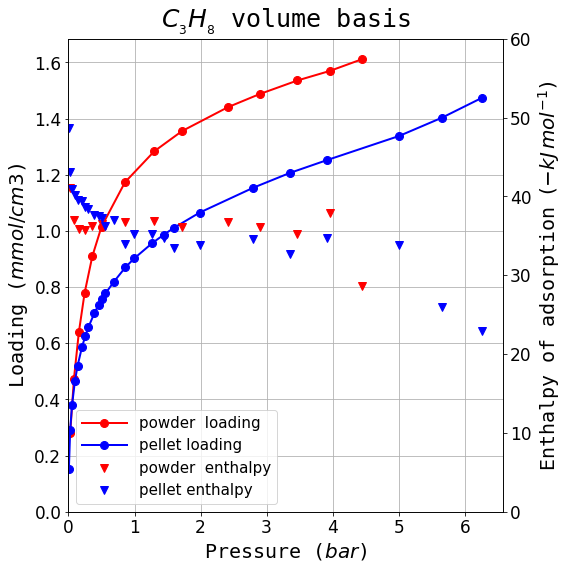
\includegraphics[width=\textwidth]{calo/UiO-66(Zr)/propane-volume-basis-iso}%
        \label{appx:fig:shaping:uio66c3h8volume}
    \end{subfigure}%
    \begin{subfigure}{0.25\textwidth}
        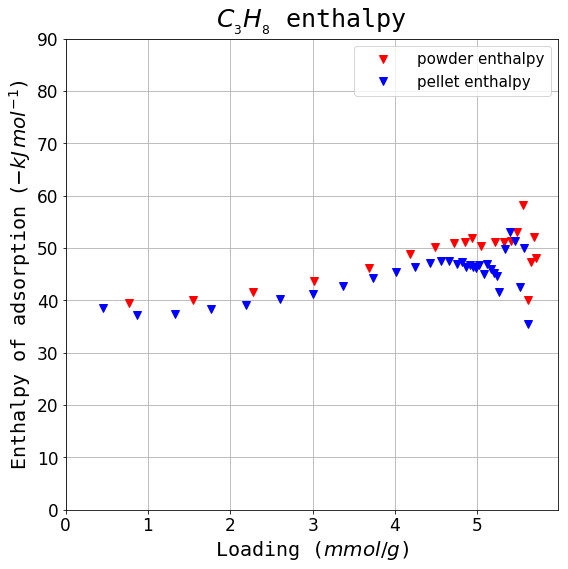
\includegraphics[width=\textwidth]{calo/UiO-66(Zr)/propane-enth}%
        \label{appx:fig:shaping:uio66c3h8enth}%
    \end{subfigure}%

    \begin{subfigure}{0.25\textwidth}
        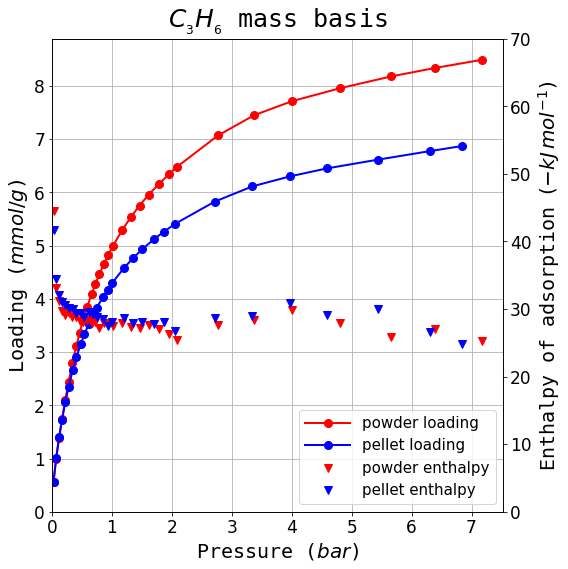
\includegraphics[width=\textwidth]{calo/UiO-66(Zr)/propene-mass-basis-iso}%
        \label{appx:fig:shaping:uio66c3h6mass}
    \end{subfigure}%
    \begin{subfigure}{0.25\textwidth}
        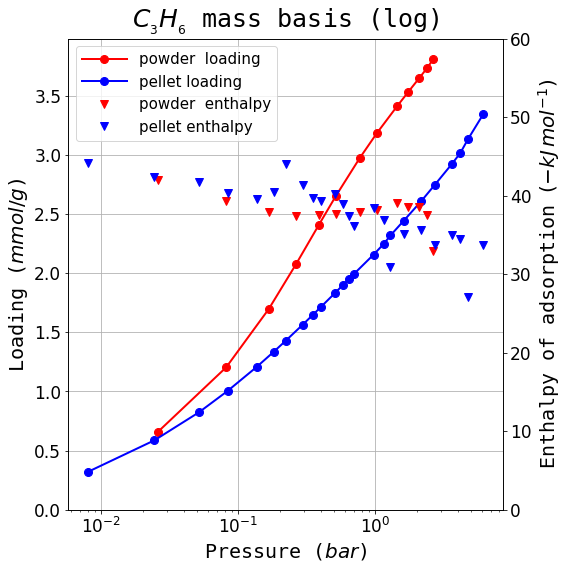
\includegraphics[width=\textwidth]{calo/UiO-66(Zr)/propene-mass-basis-log-iso}%
        \label{appx:fig:shaping:uio66c3h6masslog}
    \end{subfigure}%
    \begin{subfigure}{0.25\textwidth}
        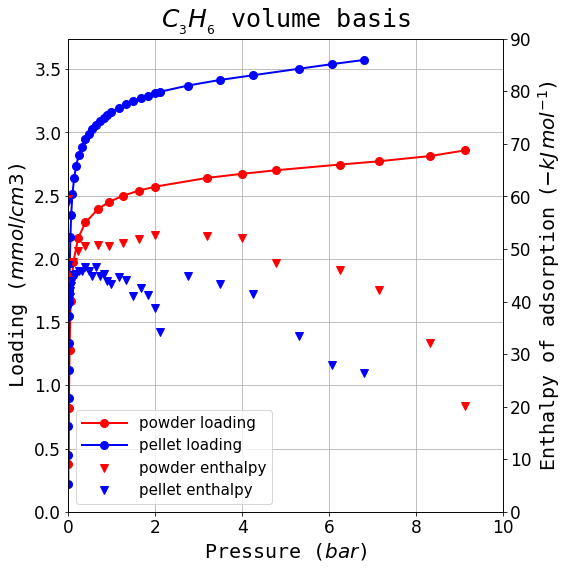
\includegraphics[width=\textwidth]{calo/UiO-66(Zr)/propene-volume-basis-iso}%
        \label{appx:fig:shaping:uio66c3h6volume}
    \end{subfigure}%
    \begin{subfigure}{0.25\textwidth}
        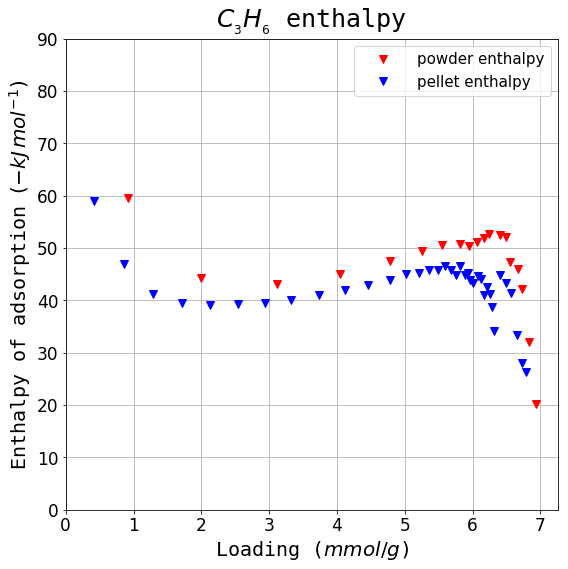
\includegraphics[width=\textwidth]{calo/UiO-66(Zr)/propene-enth}%
        \label{appx:fig:shaping:uio66c3h6enth}%
    \end{subfigure}%

    \begin{subfigure}{0.25\textwidth}
        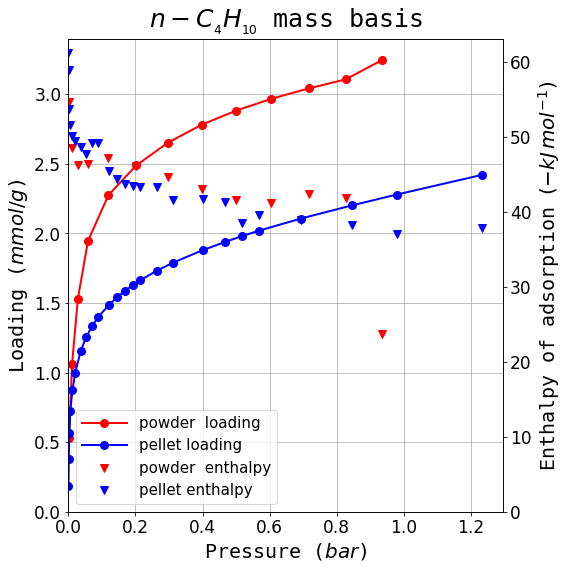
\includegraphics[width=\textwidth]{calo/UiO-66(Zr)/butane-mass-basis-iso}%
        \label{appx:fig:shaping:uio66c4h10mass}
    \end{subfigure}%
    \begin{subfigure}{0.25\textwidth}
        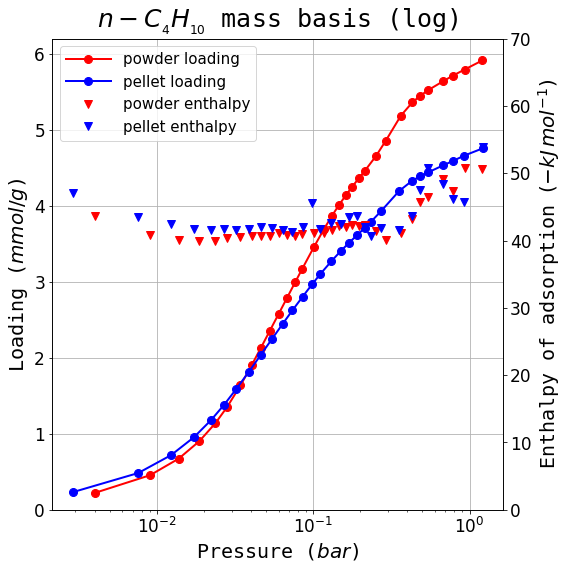
\includegraphics[width=\textwidth]{calo/UiO-66(Zr)/butane-mass-basis-log-iso}%
        \label{appx:fig:shaping:uio66c4h10masslog}
    \end{subfigure}%
    \begin{subfigure}{0.25\textwidth}
        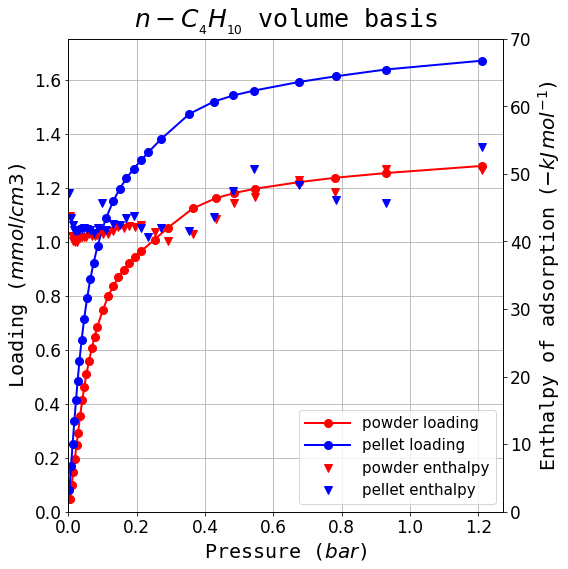
\includegraphics[width=\textwidth]{calo/UiO-66(Zr)/butane-volume-basis-iso}%
        \label{appx:fig:shaping:uio66c4h10volume}
    \end{subfigure}%
    \begin{subfigure}{0.25\textwidth}
        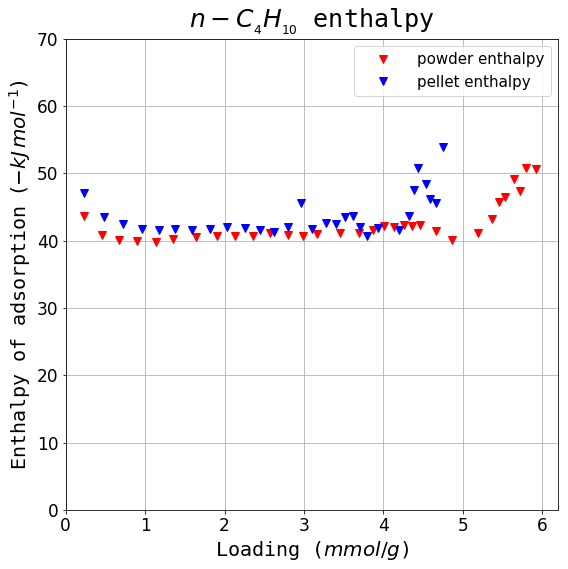
\includegraphics[width=\textwidth]{calo/UiO-66(Zr)/butane-enth}%
        \label{appx:fig:shaping:uio66c4h10enth}%
    \end{subfigure}%

    \caption{Complete isotherm and enthalpy dataset for UiO-66(Zr)}%
    \label{appx:fig:shaping:calouio66}
\end{figure}
